\section{Introduction}
\label{sec:intro}

Symbolic model checking using induction-based techniques such as IC3/PDR~\cite{Een2011:PDR}, $k$-induction~\cite{SheeranSS00}, and $k$-liveness~\cite{conf/fmcad/ClaessenS12} can often determine whether properties hold of complex finite or infinite-state systems.    Model checking tools are attractive both because they are automated, requiring little or no interaction with the user, and if the answer to a correctness query is negative, they provide a counterexample to the satisfaction of the property.  These counterexamples can be used both to illustrate subtle errors in complex hardware and software designs~\cite{hilt2013,McMillan99:compositional, Miller10:CACM} and to support automated test case generation~\cite{Whalen13:OMCDC, You15:dse}.
In the event that a property is proved, however, it is not always clear what level of assurance should be invested in the result.  Given that these kinds of analyses are performed for safety- and security-critical software, this can lead to overconfidence in the behavior of the fielded system.  Issues such as vacuity~\cite{Kupferman03:Vacuity}, incorrect environmental assumptions~\cite{Whalen07:FMICS}, and errors either in English language requirements or formalization~\cite{Pike06:axioms} can all lead to failures of ``proved'' systems.  Thus, even if proofs are established, one must approach verification with skepticism.

One substantial issue involves the level of feedback provided by the tool to the user. In most tools, when the answer to a correctness query is positive, no further information is provided. What we would like to provide is traceability information, a {\em proof core} that explains the proof, in much the same way that a counterexample explains the
negative result. This is not a new idea: UNSAT cores~\cite{zhang2003extracting} provide the same kind of information for individual SAT or
SMT queries, and this approach has been lifted to bounded analysis
for Alloy in~\cite{Torlak08:cores} and have been used for hardware model checking~\cite{jasper_gold}. What we propose is a generic and efficient
mechanism for extracting supporting information, similar to an UNSAT
core, from the proofs of safety and liveness properties using inductive techniques
such as PDR and $k$-induction, which we call an {\em inductive validity core} (IVC). Because many properties are not themselves inductive, these proof techniques introduce lemmas as part of the solving process in order to strengthen the properties and make them inductive. Our techniques allow efficient, accurate, and precise extraction of inductive validity cores even in the presence of such auxiliary lemmas.

\begin{figure}
\centering
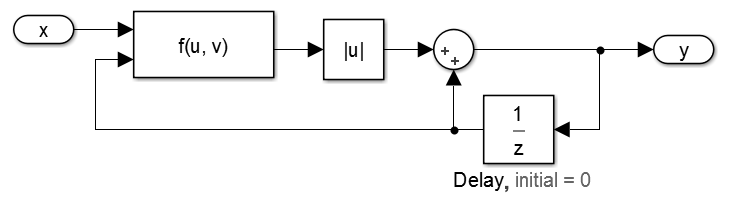
\includegraphics[width=\columnwidth]{figs/simulink.png}
{\smaller
\begin{verbatim}
node filter(x : real) returns (a, b, y : real);
let
  a = f(x, 0.0 -> pre y);
  b = if a >= 0.0 then a else -a;
  y = b + (0.0 -> pre y);
tel;
\end{verbatim}
}
\vspace{-0.1in}
\caption{Model with property $y \geq 0$, before IVC analysis}
\label{fig:ex-before}
\end{figure}


\begin{figure}[t]
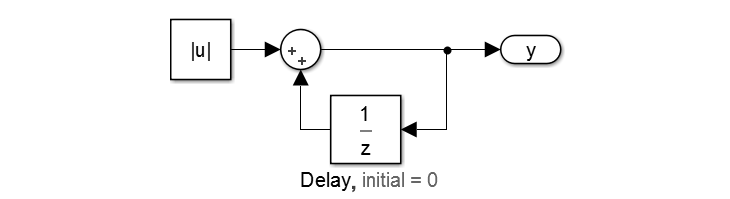
\includegraphics[width=\columnwidth]{figs/simulink-ivc.png}
{\smaller
\begin{verbatim}
node filter(x, a : real) returns (b, y : real);
let
  b = if a >= 0.0 then a else -a;
  y = b + (0.0 -> pre y);
tel;
\end{verbatim}
}
\vspace{-0.1in}
\caption{Model with property $y \geq 0$, after IVC analysis}
\label{fig:ex-after}
\end{figure}

Consider the model shown both graphically and textually in
Figure~\ref{fig:ex-before}. This model takes an input, combines it
with the previous output in some way, takes the absolute value, and
then adds this to an accumulating value. This model has the property
that the output is always non-negative, i.e., $y \geq 0$. Moreover, it
happens that this property holds regardless of the way the input is
combined with the previous output, i.e., the function $f$ in the
model. Formally, we say that the minimal inductive validity core (IVC) does
not contain that part of the model. The model reduced to a minimal IVC
is shown in Figure~\ref{fig:ex-after}. Note that traditional static
dependency analysis (i.e., a {\em backward static slice}) would not be able to
remove $f$ from the original model.  In our experiments in Section~\ref{sec:results},
we demonstrate that IVCs are much smaller and more precise than static slices.

%% \begin{itemize}
%%     \item Not sure if this should go before or after the background section with a description of Lustre.
%%     \item Need a small but interesting example.  Andrew, do any of the models that you use as jkind tests
%%         function in this way?  It would be nice to look at what we have lying around; we need something
%%         that requires invariants.
%%     \item It would also be good to have a few points of interest with the model-requirement pairing:
%%     \item \quad   vacuity due to an overconstrained environment
%%     \item \quad   definitions within the model that are irrelevant to the proof.
%%     \item Explain the model and the proof process.
%% \end{itemize}

%%  LocalWords:  IVC




IVCs are made up of a set of model elements (a notion that will be made precise in Section~\ref{sec:background}).  An IVC is {\em minimal} (MIVC) if no element can be removed while preserving provability.  Depending on the model and property to be analyzed, there is often substantial diversity between the IVCs used for proof, and there can also be a substantive difference in the size of a {\em minimal} IVC and a {\em minimum} IVC, which is the (not necessarily unique) smallest MIVC.  In this paper we describe algorithms for computing both single IVCs and {\em all} IVCs.  Once generated, IVCs can be used for many purposes in the software verification process, including at least the following:
%\mike{There is something weird with the description environment so I am manually spacing it}

\noindent \textbf{Traceability:} Certification standards for safety-critical systems (e.g.,~\cite{DO178C, MOD:00-55}) usually require {\em traceability matrices} that map high-level requirements to lower-level requirements and (eventually) leaf-level requirements to code or models.  Current traceability approaches involve either manual mappings between requirements and code/models~\cite{SimulinkTraceability} or a heuristic approach involving natural language processing~\cite{Keenan12:Tracelab}.  Both of these approaches tend to be inaccurate.  For functional properties that can be proven with inductive model checkers, inductive validity cores can provide accurate traceability matrices with no user effort.

\noindent \textbf{Vacuity detection:} The idea of syntactic vacuity detection (checking whether all subformulae within a property are necessary for its validity) has been well studied~\cite{Kupferman03:Vacuity}.   IVCs allow a generalized notion of vacuity that can indicate weak or mis-specified properties even when a property is syntactically non-vacuous.   This kind of mis-specification occurs regularly, especially when variables computed by the model are used as elements of antecedents in implicative properties.

\noindent \textbf{Coverage analysis:} Closely related to vacuity detection is the idea of {\em coverage analysis}, e.g., are all atoms in the model necessary for at least one of the properties proven about the model?  Several different notions of coverage have been proposed~\cite{chockler_coverage_2003, kupferman_theory_2008}, but these tend to be very expensive to compute, and in some cases, can only be used for certain kinds of models (e.g., checking can only be performed on non-vacuous models for~\cite{kupferman_theory_2008}).

\noindent \textbf{Symbolic Simulation / Test Case Generation:} Model checkers are now often used for symbolic simulation and structural-coverage-based test case generation~\cite{SimulinkDesignVerifier,Whalen13:OMCDC}.  For either of these purposes, the model checker is supposed to produce a witness trace for a given coverage obligation using a ``trap property'' which is expected to be falsifiable.  In systems of sufficient size, there is often ``dead code'' that cannot ever be reached.  In this case, a proof of non-reachability is produced, and the IVC provides the reason why this code is unreachable.

\noindent \textbf{Design Optimization:} Synthesis tools can benefit from MIVCs in the process of transforming an abstract behavior into a design implementation. A practical way of calculating all MIVCs allows to find a minimum set of design elements (optimal implementation) for a certain behavior. Such optimizations can be performed at different levels of synthesis.

\noindent \textbf{Impact Analysis:} Given a single (or for more accurate results, all) MIVCs, it is possible to determine which requirements may be falsified by changes to the model.  This analysis allows for selective regression verification of tests and proofs: if there are alternate proof paths that do not require the modified portions of the model, then the requirement does not need to be re-verified.

To be useful for these tasks, the generation process must be efficient and the generated IVC must be accurate and precise (that is, sound and close to minimal).  The requirement for accuracy is obvious; otherwise the ``minimal'' set of model elements is no longer sufficient to produce a proof, so it no longer meets our IVC definition.  Minimality is important because (for traceability) we do not want unnecessary model elements in the trace matrix, and (for completeness) it may give us a false level of confidence that we have enough requirements.

The goal of this paper is to prevent a definitive and comprehensive explanation of algorithms and applications for inductive validity cores.  It provides a unified treatment of material from four conference papers~\cite{Ghass16,Murugesan16:renext,Ghass17Cov,Ghass17AllIVCs}.  Additionally, it contains (1) a significantly larger experiment than previous work, both in terms of the number of models (660 vs. 476) that is a superset of a large benchmark suite used to evaluate model checking tools in~\cite{piskac2016}, with the number of ``large'' models (containing more than 100 equations) enlarged from 81 to 130, (2) an expanded treatment of coverage metrics based on IVCs and their relations to previous metrics, (3) a discussion of {\em granularity} of model elements and how this affects traceability information, especially in regards to coverage of requirements, and (4) revised, more detailed proofs that fix a handful of clerical mistakes in previous papers.


The remainder of the paper is organized as follows: Section~\ref{sec:example} provides a running example that will be used to illustrate concepts in the remainder of the paper.  Section~\ref{sec:background} provides formal preliminaries.  Section~\ref{sec:ivc} describes inductive validity cores and provides algorithms for both generating a single IVC and all IVCs.  Section~\ref{sec:impl} describes the implementation.  Section~\ref{sec:experiment} describes an experiment that examines fitness for purpose of the different IVC algorithms.  Section~\ref{sec:apps} describes applications of IVCs for different software engineering purposes.   Section~\ref{sec:disc} provides a discussion of IVCs and their utility for different tasks.  Section~\ref{sec:conc} concludes.

%The remainder of the paper is organized as follows...
